\chapter{Object and Event Selection}
\label{chap:ObjEvt}

%%%%%%%%%%%%%%%%%%%%%%%%%%%%%%%%%%%%%%%%%%%%%%%%%%
%%%%%%%%%%%%%%%%%%%%%%%%%%%%%%%%%%%%%%%%%%%%%%%%%%
\section{Object Selection}
\label{sec:Obj}

%%%%%%%%%%%%%%%%%%%%%%%%%%%%%%%%%%%%%%%%%%%%%%%%%%
\subsection{Electrons and Muons}
\label{subsec:EandM}

An updated version of the \TOP\cite{CMS:2023ftu} is used to select \emph{prompt} leptons.
%%%%%%%%%%%%%%%%%%%%%%%%%%%%%%%%%%%%%%%%%%%%%%%%%%
\subsection{Hadronic Taus}
\label{subsec:Taus}

A \ac{NN}-based algorithm~\cite{CMS:2022prd} is used to identify hadronic tau leptons.
%%%%%%%%%%%%%%%%%%%%%%%%%%%%%%%%%%%%%%%%%%%%%%%%%%
\subsection{Jets and MET}
\label{subsec:JME}


%%%%%%%%%%%%%%%%%%%%%%%%%%%%%%%%%%%%%%%%%%%%%%%%%%
%%%%%%%%%%%%%%%%%%%%%%%%%%%%%%%%%%%%%%%%%%%%%%%%%%
\section{Event Selection}
\label{sec:Evt}

\subsection{Event Categorization}
\label{subsec:Cat}

\begin{figure}[tbh!]
 \begin{center}
 \begin{tabular}{c}
 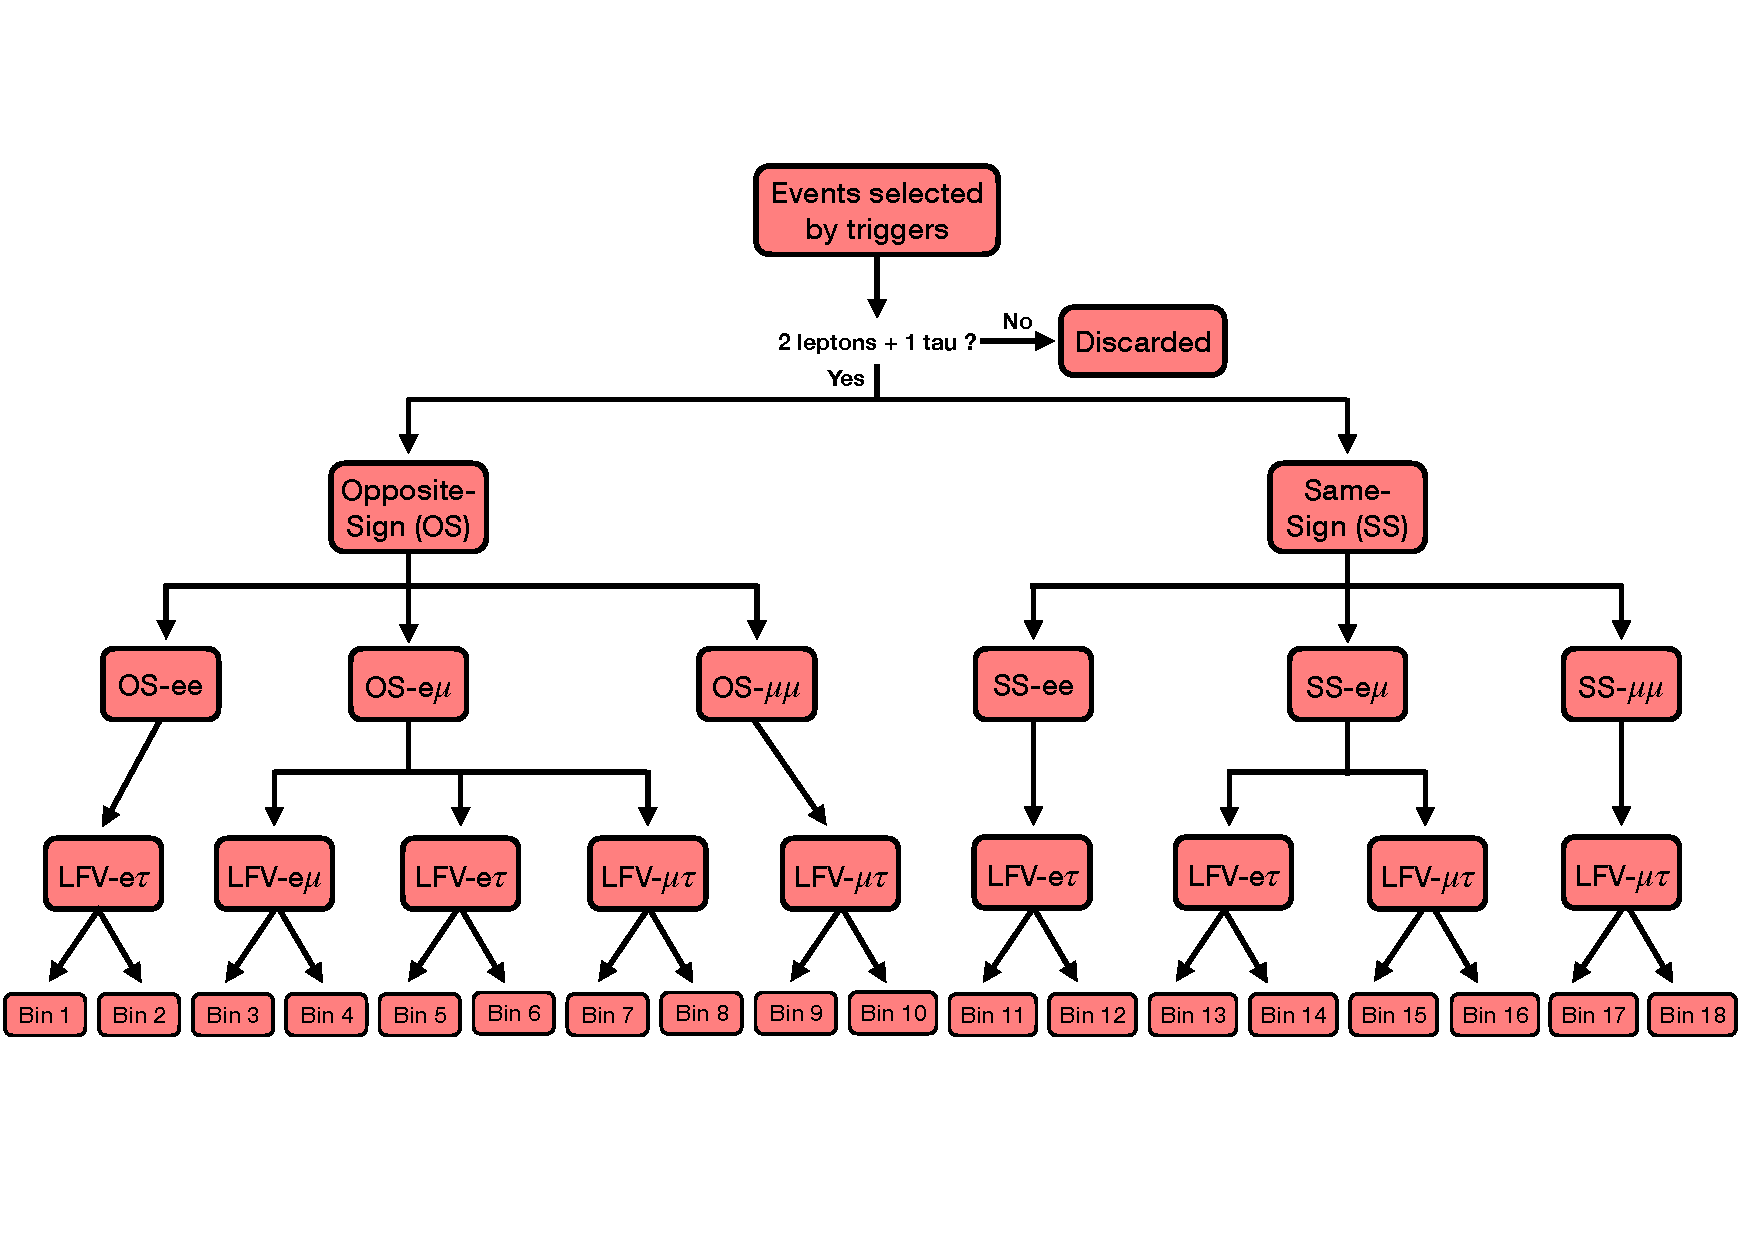
\includegraphics[width=\textwidth]{figures/Part4/ObjEvt/SRFlowChart}
 \end{tabular}
 \caption{XX}
 \label{fig:EvtCat}
 \end{center}
 \end{figure}
%%%%%%%%%%%%%%%%%%%%%%%%%%%%%%%%%%%%%%%%%%%%%%%%%%

\subsection{Signal Region}
\label{subsec:SR}

\begin{figure}[tbh!]
 \begin{center}
 \begin{tabular}{c}
 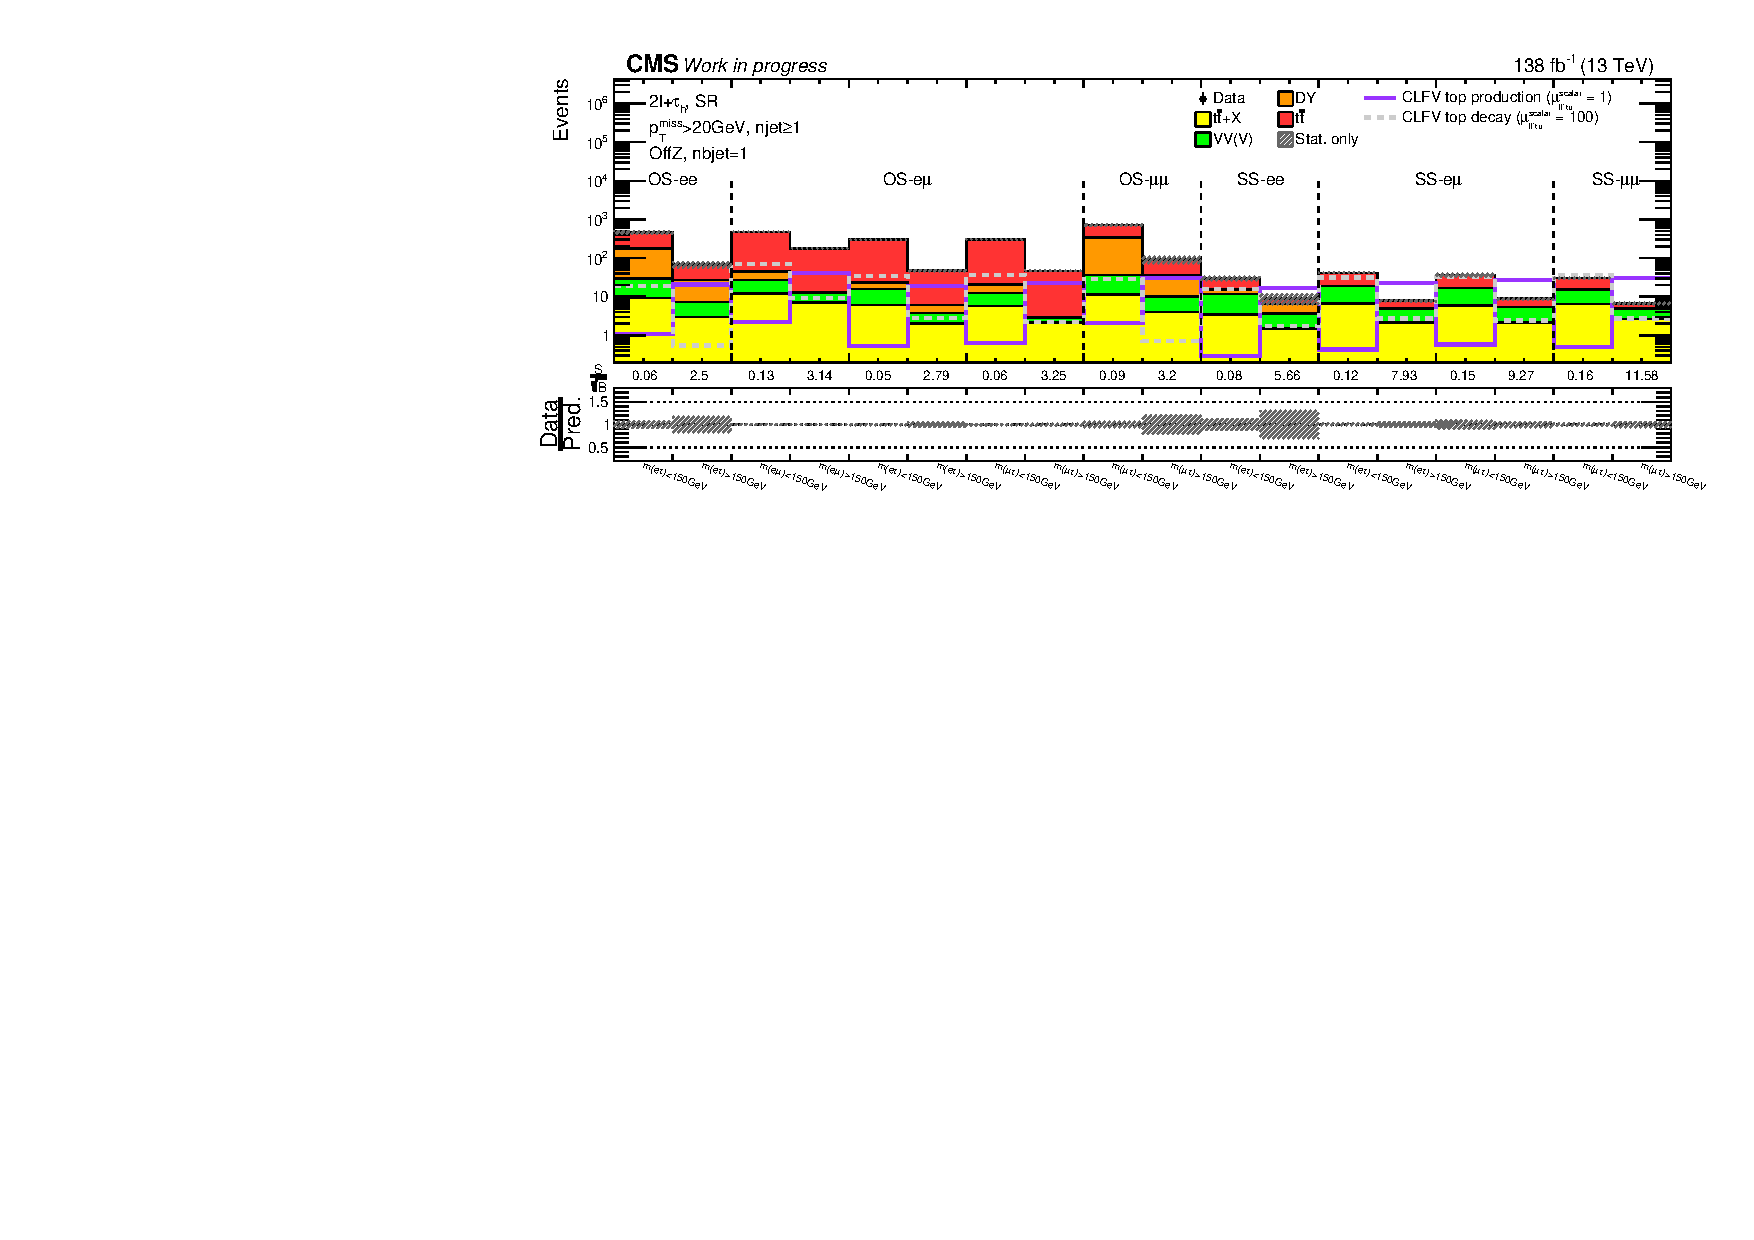
\includegraphics[width=\textwidth]{figures/Part4/ObjEvt/Summary_llOffZMetg20B1}
 \end{tabular}
 \caption{XX}
 \label{fig:Summary}
 \end{center}
 \end{figure}
 
 \begin{figure}[tbh!]
 \begin{center}
 \begin{tabular}{c}
 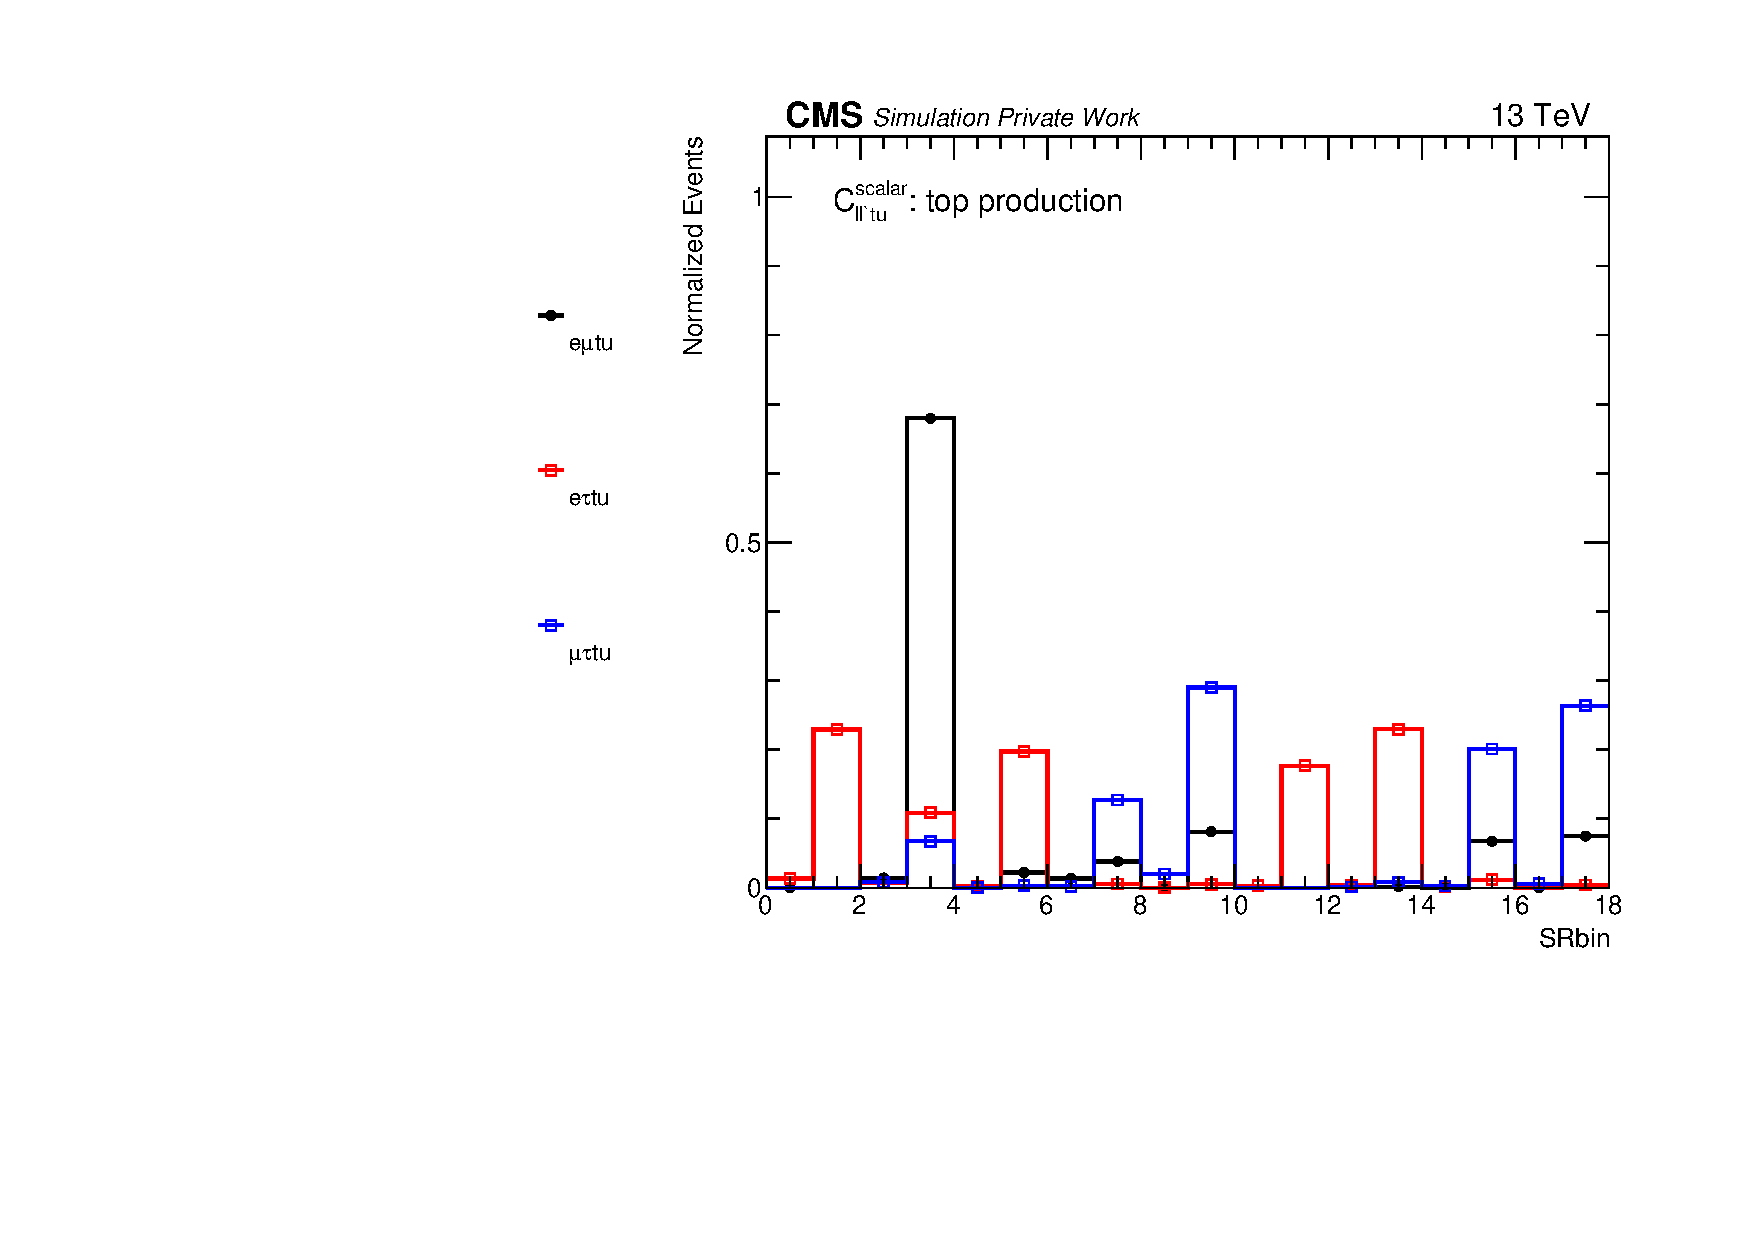
\includegraphics[width=\textwidth]{figures/Part4/ObjEvt/SRbin}
 \end{tabular}
 \caption{XX}
 \label{fig:Summary}
 \end{center}
 \end{figure}
 
 \begin{figure}[tbh!]
 \begin{center}
 \begin{tabular}{ccc}
 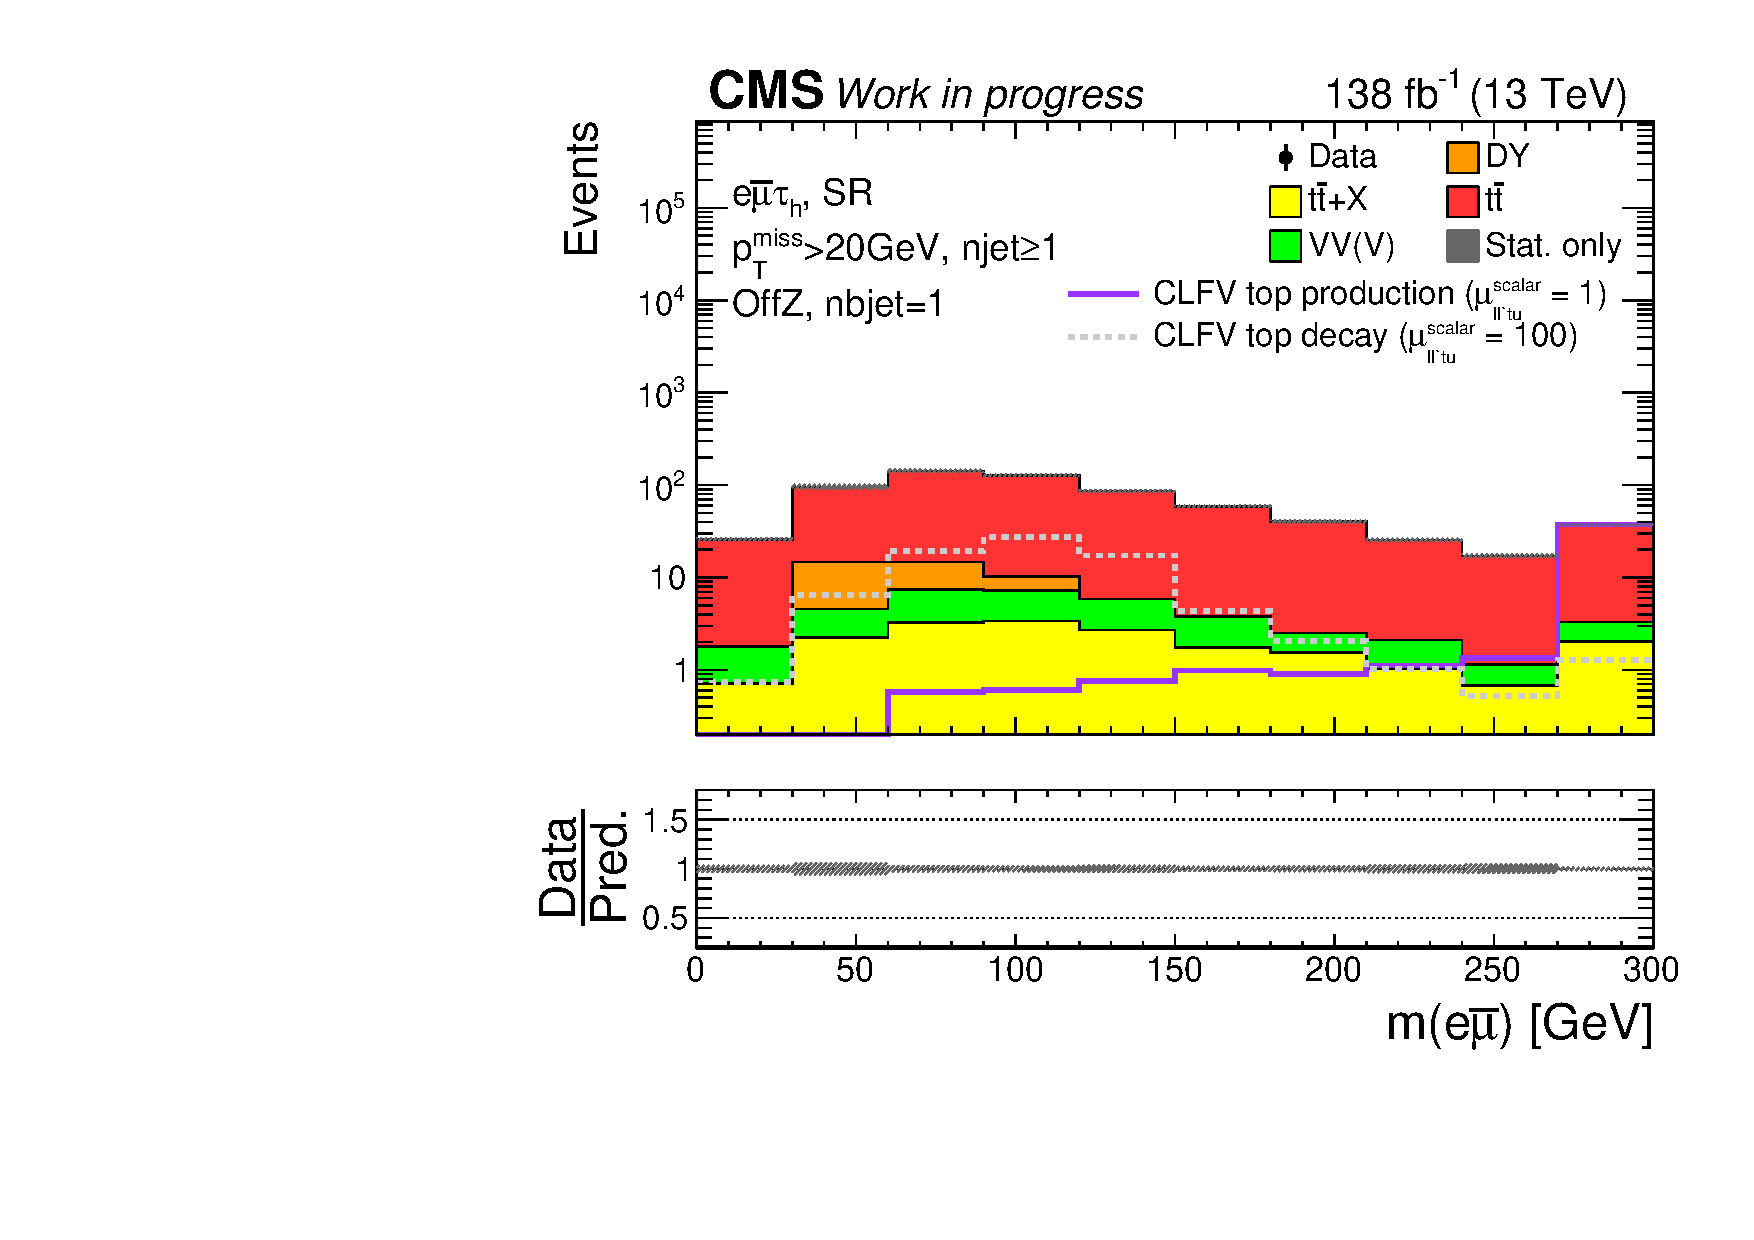
\includegraphics[width=0.33\textwidth]{figures/Part4/ObjEvt/LFVemuM}&
  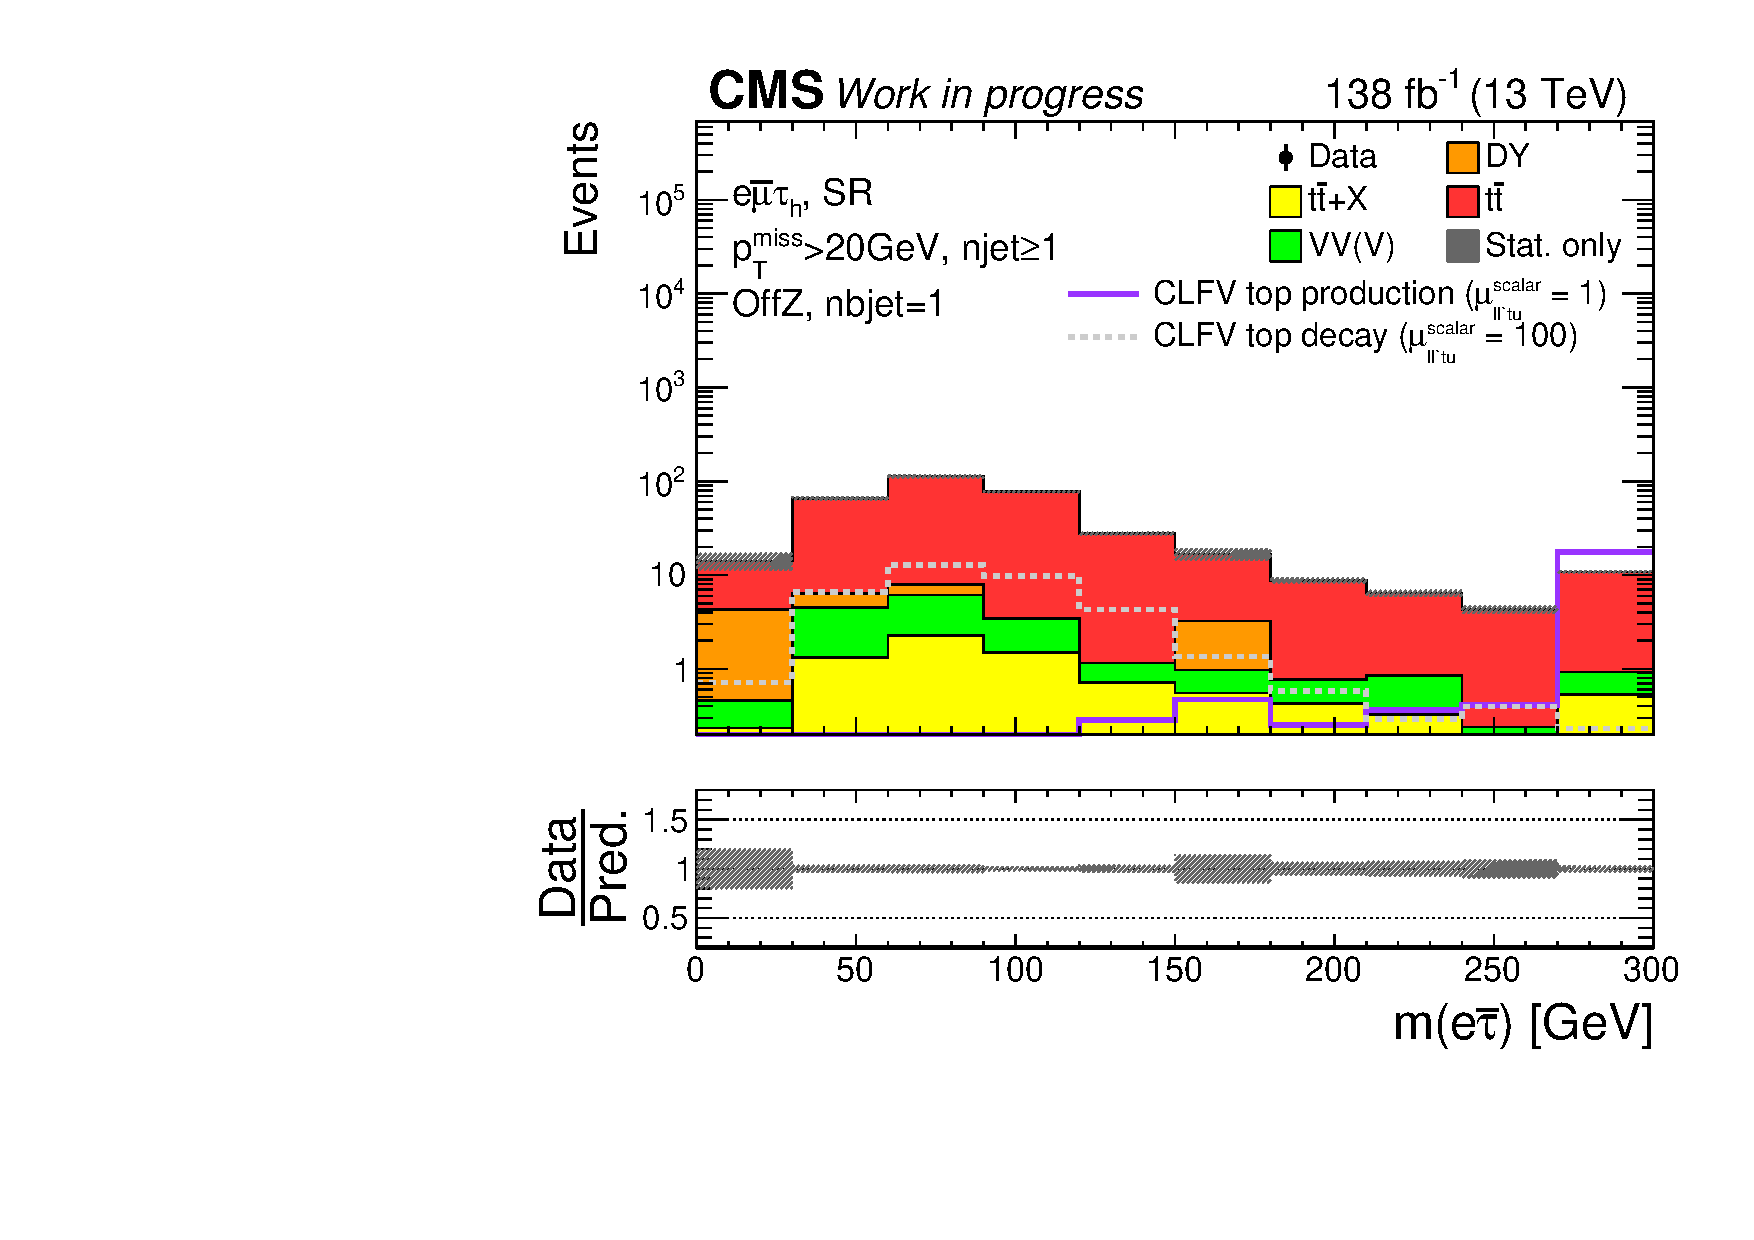
\includegraphics[width=0.33\textwidth]{figures/Part4/ObjEvt/LFVetaM}&
   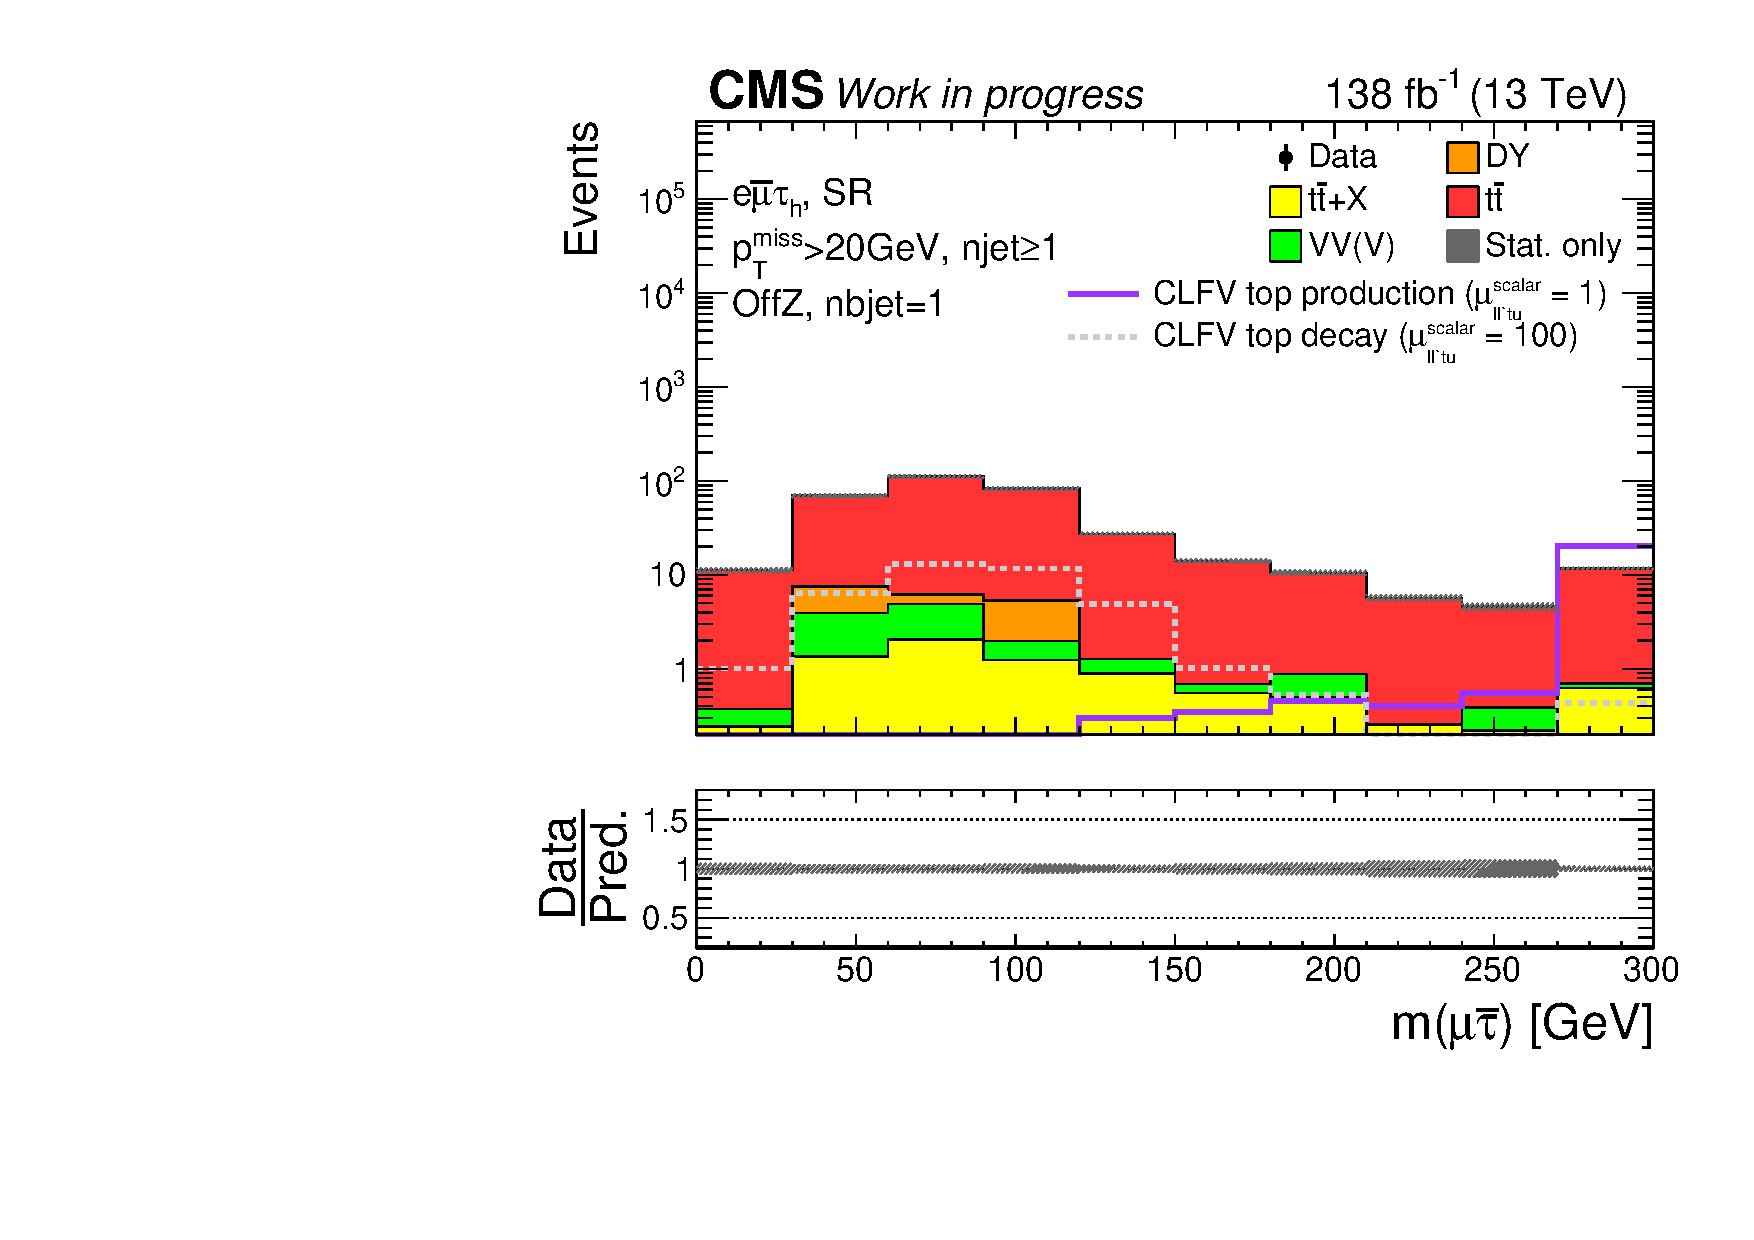
\includegraphics[width=0.33\textwidth]{figures/Part4/ObjEvt/LFVmutaM}\\
 \end{tabular}
 \caption{XX}
 \label{fig:Summary}
 \end{center}
 \end{figure}
%%%%%%%%%%%%%%%%%%%%%%%%%%%%%%%%%%%%%%%%%%%%%%%%%%

\subsection{Drell-Yan Control Region}
\label{subsec:CR}

 \begin{figure}[tbh!]
 \begin{center}
 \begin{tabular}{cc}
 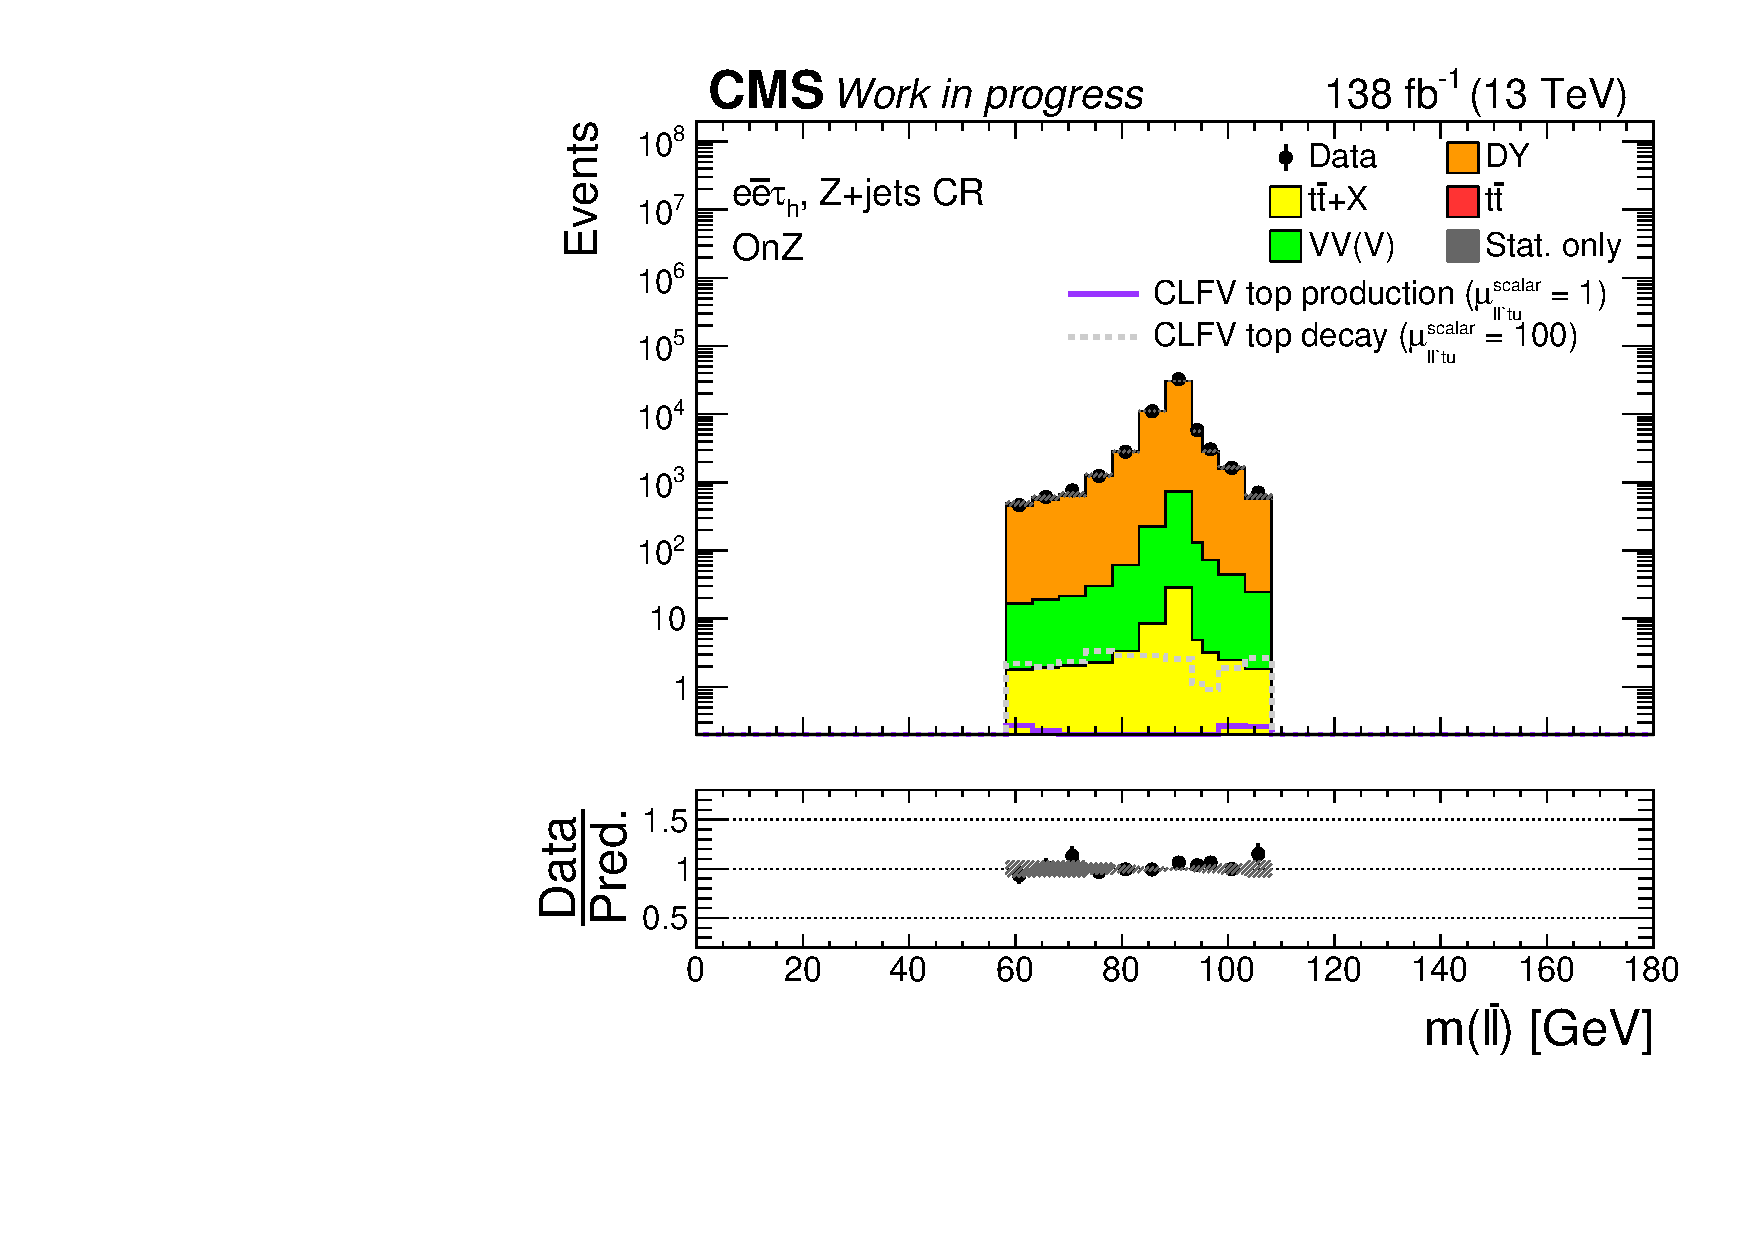
\includegraphics[width=0.48\textwidth]{figures/Part4/ObjEvt/llM_OnZ_ee}&
 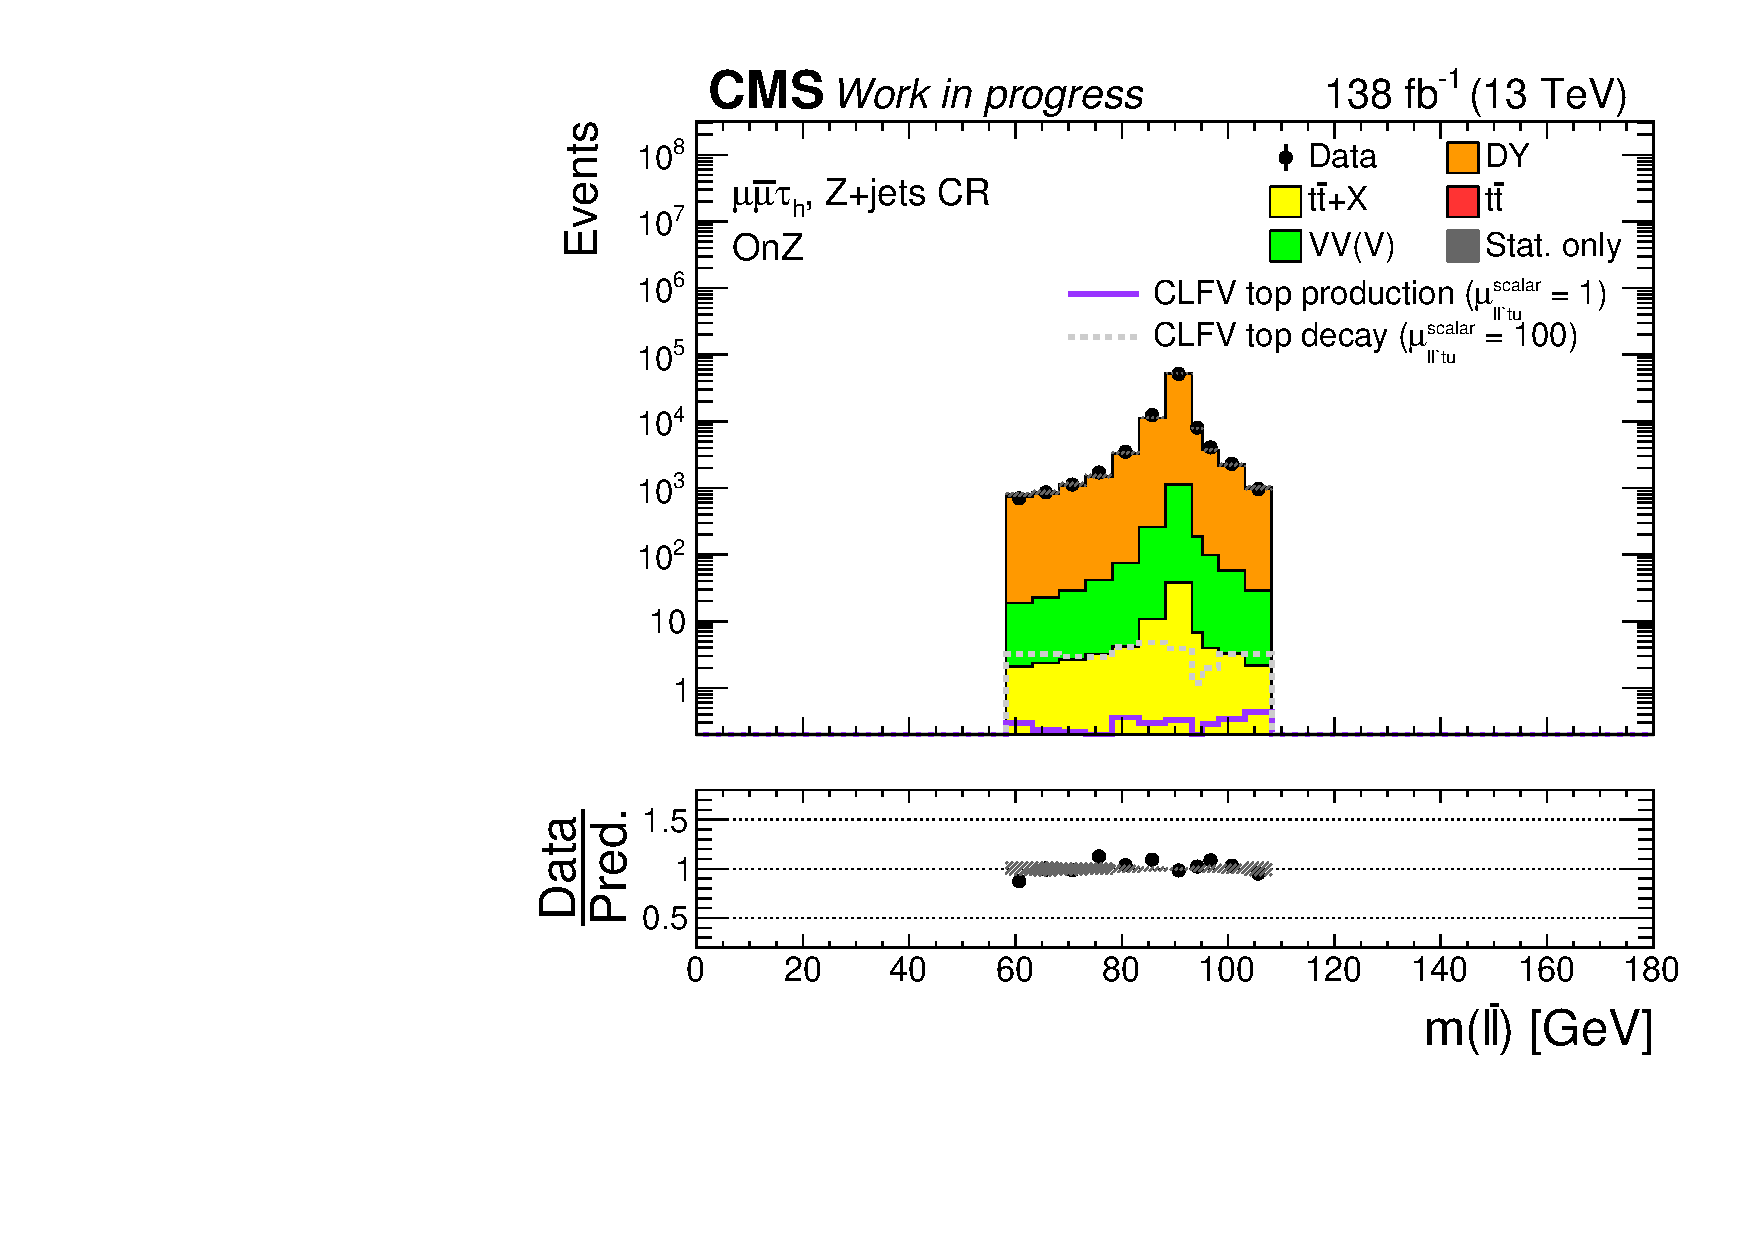
\includegraphics[width=0.48\textwidth]{figures/Part4/ObjEvt/llM_OnZ_mumu}\\
  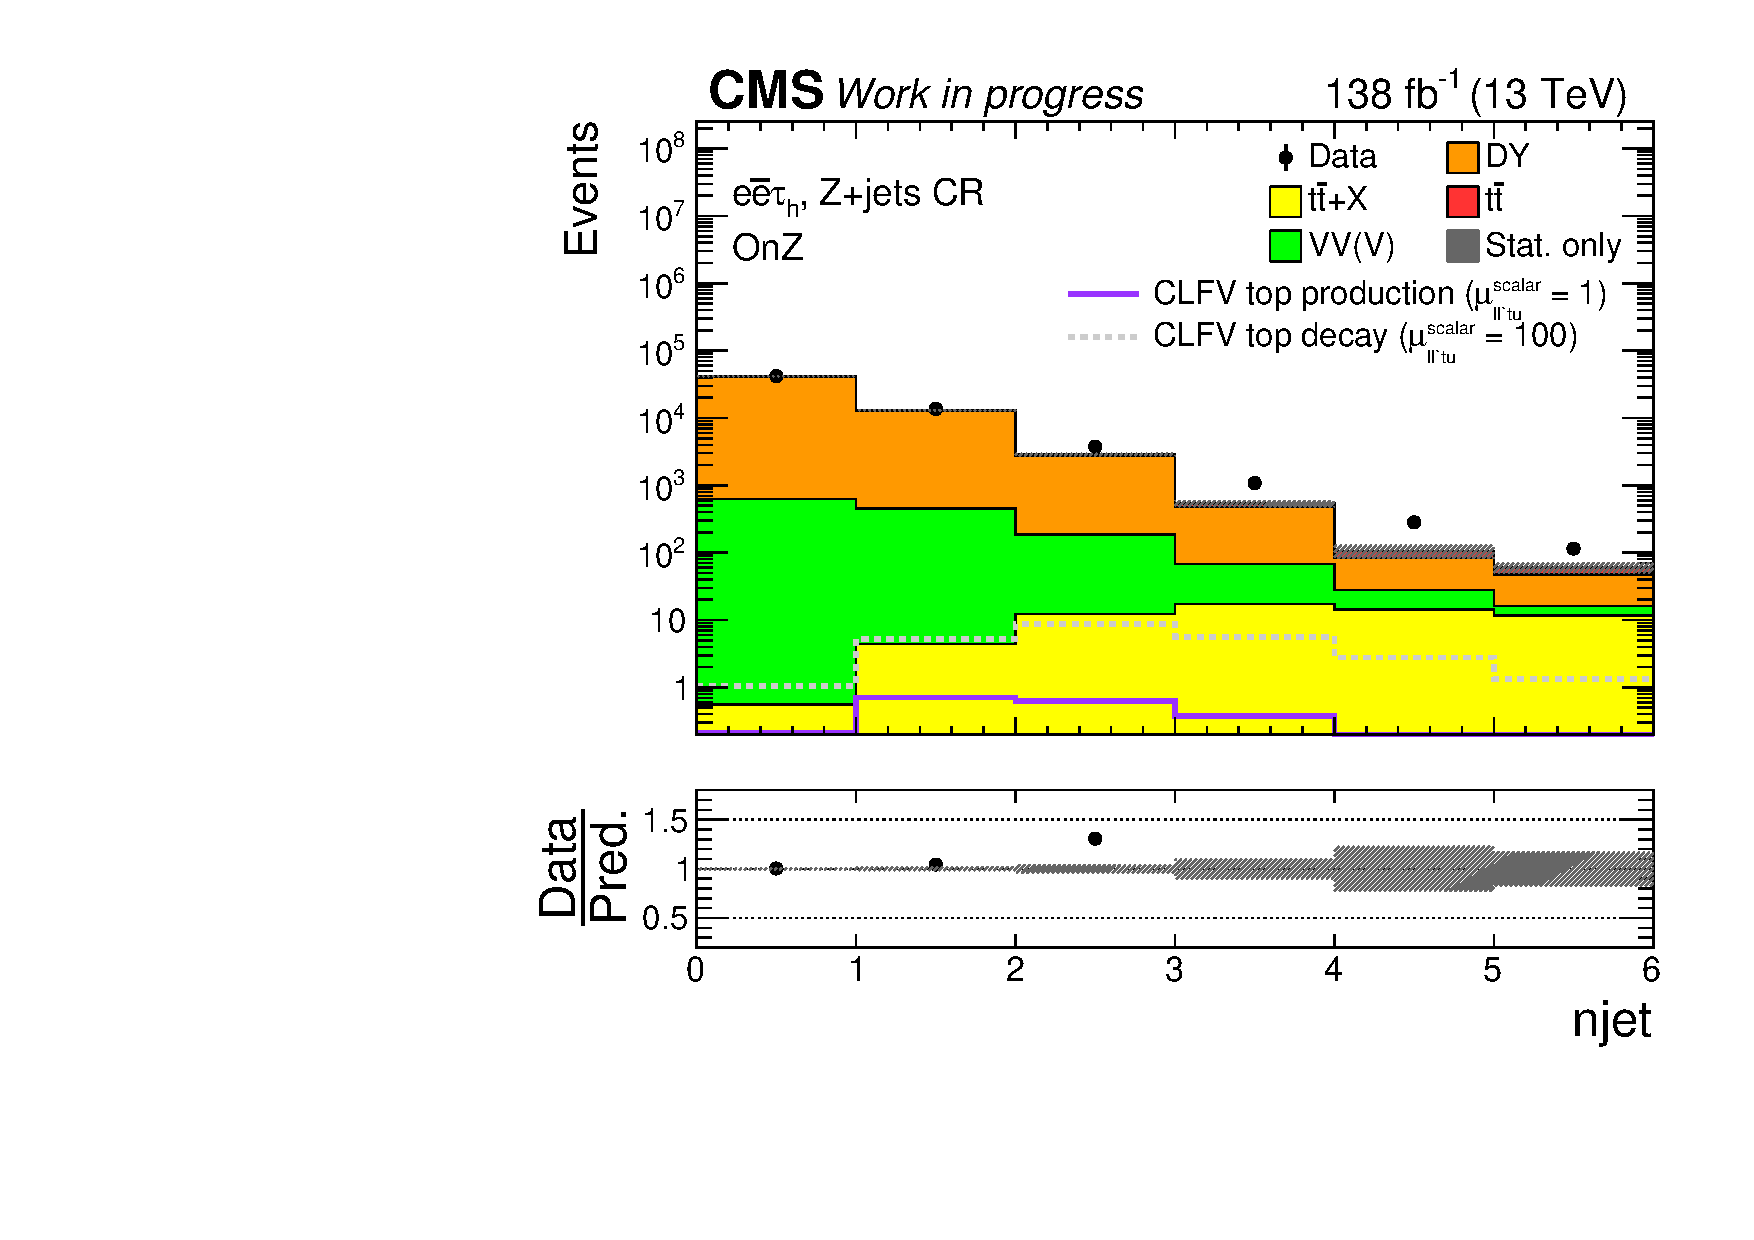
\includegraphics[width=0.48\textwidth]{figures/Part4/ObjEvt/njet_OnZ_ee}&
 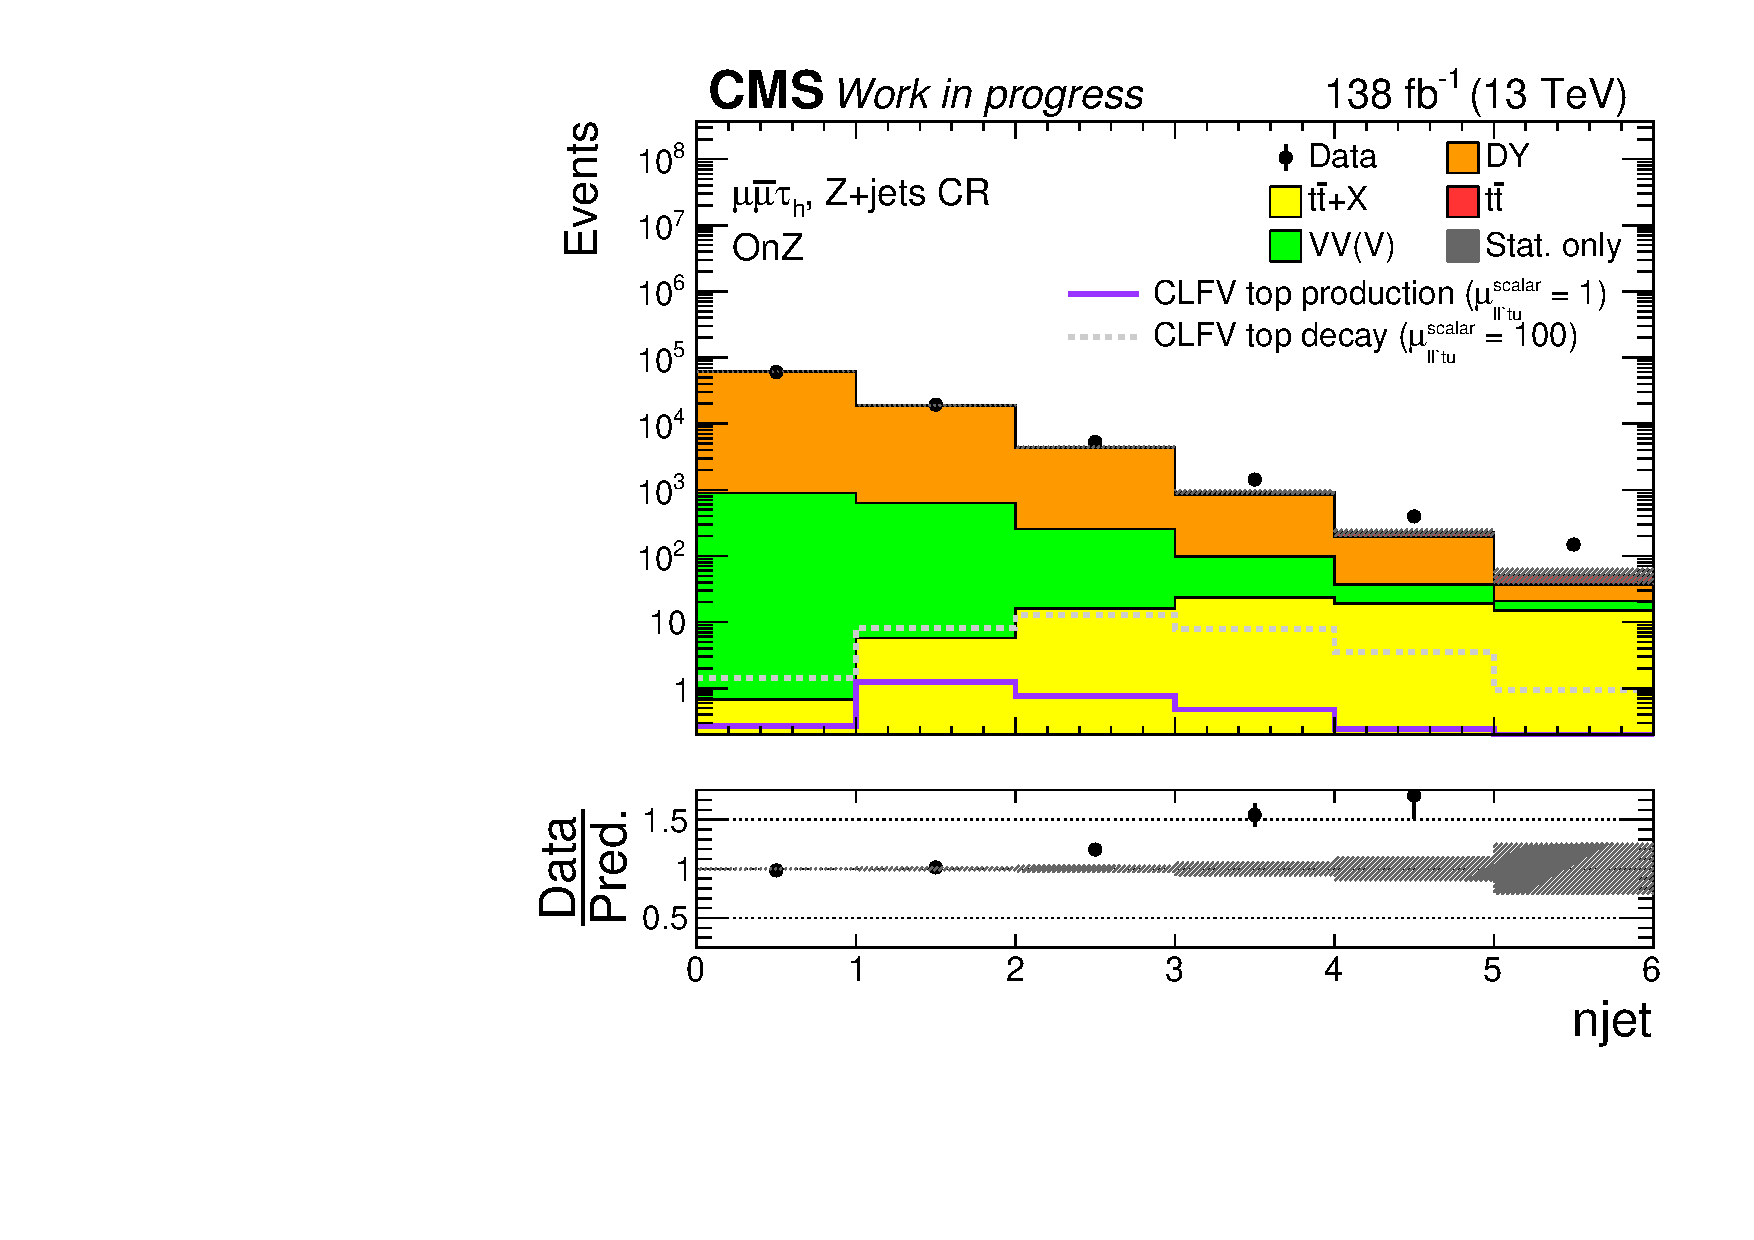
\includegraphics[width=0.48\textwidth]{figures/Part4/ObjEvt/njet_OnZ_mumu}\\
 \end{tabular}
 \caption{XX}
 \label{fig:DY_CR}
 \end{center}
 \end{figure}
%%%%%%%%%%%%%%%%%%%%%%%%%%%%%%%%%%%%%%%%%%%%%%%%%%

